% Options for packages loaded elsewhere
\PassOptionsToPackage{unicode}{hyperref}
\PassOptionsToPackage{hyphens}{url}
\PassOptionsToPackage{dvipsnames,svgnames,x11names}{xcolor}
%
\documentclass[
  letterpaper,
  DIV=11,
  numbers=noendperiod]{scrreprt}

\usepackage{amsmath,amssymb}
\usepackage{iftex}
\ifPDFTeX
  \usepackage[T1]{fontenc}
  \usepackage[utf8]{inputenc}
  \usepackage{textcomp} % provide euro and other symbols
\else % if luatex or xetex
  \usepackage{unicode-math}
  \defaultfontfeatures{Scale=MatchLowercase}
  \defaultfontfeatures[\rmfamily]{Ligatures=TeX,Scale=1}
\fi
\usepackage{lmodern}
\ifPDFTeX\else  
    % xetex/luatex font selection
\fi
% Use upquote if available, for straight quotes in verbatim environments
\IfFileExists{upquote.sty}{\usepackage{upquote}}{}
\IfFileExists{microtype.sty}{% use microtype if available
  \usepackage[]{microtype}
  \UseMicrotypeSet[protrusion]{basicmath} % disable protrusion for tt fonts
}{}
\makeatletter
\@ifundefined{KOMAClassName}{% if non-KOMA class
  \IfFileExists{parskip.sty}{%
    \usepackage{parskip}
  }{% else
    \setlength{\parindent}{0pt}
    \setlength{\parskip}{6pt plus 2pt minus 1pt}}
}{% if KOMA class
  \KOMAoptions{parskip=half}}
\makeatother
\usepackage{xcolor}
\setlength{\emergencystretch}{3em} % prevent overfull lines
\setcounter{secnumdepth}{-\maxdimen} % remove section numbering
% Make \paragraph and \subparagraph free-standing
\makeatletter
\ifx\paragraph\undefined\else
  \let\oldparagraph\paragraph
  \renewcommand{\paragraph}{
    \@ifstar
      \xxxParagraphStar
      \xxxParagraphNoStar
  }
  \newcommand{\xxxParagraphStar}[1]{\oldparagraph*{#1}\mbox{}}
  \newcommand{\xxxParagraphNoStar}[1]{\oldparagraph{#1}\mbox{}}
\fi
\ifx\subparagraph\undefined\else
  \let\oldsubparagraph\subparagraph
  \renewcommand{\subparagraph}{
    \@ifstar
      \xxxSubParagraphStar
      \xxxSubParagraphNoStar
  }
  \newcommand{\xxxSubParagraphStar}[1]{\oldsubparagraph*{#1}\mbox{}}
  \newcommand{\xxxSubParagraphNoStar}[1]{\oldsubparagraph{#1}\mbox{}}
\fi
\makeatother

\usepackage{color}
\usepackage{fancyvrb}
\newcommand{\VerbBar}{|}
\newcommand{\VERB}{\Verb[commandchars=\\\{\}]}
\DefineVerbatimEnvironment{Highlighting}{Verbatim}{commandchars=\\\{\}}
% Add ',fontsize=\small' for more characters per line
\usepackage{framed}
\definecolor{shadecolor}{RGB}{241,243,245}
\newenvironment{Shaded}{\begin{snugshade}}{\end{snugshade}}
\newcommand{\AlertTok}[1]{\textcolor[rgb]{0.68,0.00,0.00}{#1}}
\newcommand{\AnnotationTok}[1]{\textcolor[rgb]{0.37,0.37,0.37}{#1}}
\newcommand{\AttributeTok}[1]{\textcolor[rgb]{0.40,0.45,0.13}{#1}}
\newcommand{\BaseNTok}[1]{\textcolor[rgb]{0.68,0.00,0.00}{#1}}
\newcommand{\BuiltInTok}[1]{\textcolor[rgb]{0.00,0.23,0.31}{#1}}
\newcommand{\CharTok}[1]{\textcolor[rgb]{0.13,0.47,0.30}{#1}}
\newcommand{\CommentTok}[1]{\textcolor[rgb]{0.37,0.37,0.37}{#1}}
\newcommand{\CommentVarTok}[1]{\textcolor[rgb]{0.37,0.37,0.37}{\textit{#1}}}
\newcommand{\ConstantTok}[1]{\textcolor[rgb]{0.56,0.35,0.01}{#1}}
\newcommand{\ControlFlowTok}[1]{\textcolor[rgb]{0.00,0.23,0.31}{\textbf{#1}}}
\newcommand{\DataTypeTok}[1]{\textcolor[rgb]{0.68,0.00,0.00}{#1}}
\newcommand{\DecValTok}[1]{\textcolor[rgb]{0.68,0.00,0.00}{#1}}
\newcommand{\DocumentationTok}[1]{\textcolor[rgb]{0.37,0.37,0.37}{\textit{#1}}}
\newcommand{\ErrorTok}[1]{\textcolor[rgb]{0.68,0.00,0.00}{#1}}
\newcommand{\ExtensionTok}[1]{\textcolor[rgb]{0.00,0.23,0.31}{#1}}
\newcommand{\FloatTok}[1]{\textcolor[rgb]{0.68,0.00,0.00}{#1}}
\newcommand{\FunctionTok}[1]{\textcolor[rgb]{0.28,0.35,0.67}{#1}}
\newcommand{\ImportTok}[1]{\textcolor[rgb]{0.00,0.46,0.62}{#1}}
\newcommand{\InformationTok}[1]{\textcolor[rgb]{0.37,0.37,0.37}{#1}}
\newcommand{\KeywordTok}[1]{\textcolor[rgb]{0.00,0.23,0.31}{\textbf{#1}}}
\newcommand{\NormalTok}[1]{\textcolor[rgb]{0.00,0.23,0.31}{#1}}
\newcommand{\OperatorTok}[1]{\textcolor[rgb]{0.37,0.37,0.37}{#1}}
\newcommand{\OtherTok}[1]{\textcolor[rgb]{0.00,0.23,0.31}{#1}}
\newcommand{\PreprocessorTok}[1]{\textcolor[rgb]{0.68,0.00,0.00}{#1}}
\newcommand{\RegionMarkerTok}[1]{\textcolor[rgb]{0.00,0.23,0.31}{#1}}
\newcommand{\SpecialCharTok}[1]{\textcolor[rgb]{0.37,0.37,0.37}{#1}}
\newcommand{\SpecialStringTok}[1]{\textcolor[rgb]{0.13,0.47,0.30}{#1}}
\newcommand{\StringTok}[1]{\textcolor[rgb]{0.13,0.47,0.30}{#1}}
\newcommand{\VariableTok}[1]{\textcolor[rgb]{0.07,0.07,0.07}{#1}}
\newcommand{\VerbatimStringTok}[1]{\textcolor[rgb]{0.13,0.47,0.30}{#1}}
\newcommand{\WarningTok}[1]{\textcolor[rgb]{0.37,0.37,0.37}{\textit{#1}}}

\providecommand{\tightlist}{%
  \setlength{\itemsep}{0pt}\setlength{\parskip}{0pt}}\usepackage{longtable,booktabs,array}
\usepackage{calc} % for calculating minipage widths
% Correct order of tables after \paragraph or \subparagraph
\usepackage{etoolbox}
\makeatletter
\patchcmd\longtable{\par}{\if@noskipsec\mbox{}\fi\par}{}{}
\makeatother
% Allow footnotes in longtable head/foot
\IfFileExists{footnotehyper.sty}{\usepackage{footnotehyper}}{\usepackage{footnote}}
\makesavenoteenv{longtable}
\usepackage{graphicx}
\makeatletter
\newsavebox\pandoc@box
\newcommand*\pandocbounded[1]{% scales image to fit in text height/width
  \sbox\pandoc@box{#1}%
  \Gscale@div\@tempa{\textheight}{\dimexpr\ht\pandoc@box+\dp\pandoc@box\relax}%
  \Gscale@div\@tempb{\linewidth}{\wd\pandoc@box}%
  \ifdim\@tempb\p@<\@tempa\p@\let\@tempa\@tempb\fi% select the smaller of both
  \ifdim\@tempa\p@<\p@\scalebox{\@tempa}{\usebox\pandoc@box}%
  \else\usebox{\pandoc@box}%
  \fi%
}
% Set default figure placement to htbp
\def\fps@figure{htbp}
\makeatother

\KOMAoption{captions}{tableheading}
\makeatletter
\@ifpackageloaded{caption}{}{\usepackage{caption}}
\AtBeginDocument{%
\ifdefined\contentsname
  \renewcommand*\contentsname{Table of contents}
\else
  \newcommand\contentsname{Table of contents}
\fi
\ifdefined\listfigurename
  \renewcommand*\listfigurename{List of Figures}
\else
  \newcommand\listfigurename{List of Figures}
\fi
\ifdefined\listtablename
  \renewcommand*\listtablename{List of Tables}
\else
  \newcommand\listtablename{List of Tables}
\fi
\ifdefined\figurename
  \renewcommand*\figurename{Figure}
\else
  \newcommand\figurename{Figure}
\fi
\ifdefined\tablename
  \renewcommand*\tablename{Table}
\else
  \newcommand\tablename{Table}
\fi
}
\@ifpackageloaded{float}{}{\usepackage{float}}
\floatstyle{ruled}
\@ifundefined{c@chapter}{\newfloat{codelisting}{h}{lop}}{\newfloat{codelisting}{h}{lop}[chapter]}
\floatname{codelisting}{Listing}
\newcommand*\listoflistings{\listof{codelisting}{List of Listings}}
\makeatother
\makeatletter
\makeatother
\makeatletter
\@ifpackageloaded{caption}{}{\usepackage{caption}}
\@ifpackageloaded{subcaption}{}{\usepackage{subcaption}}
\makeatother

\usepackage{bookmark}

\IfFileExists{xurl.sty}{\usepackage{xurl}}{} % add URL line breaks if available
\urlstyle{same} % disable monospaced font for URLs
\hypersetup{
  pdftitle={Week2-Exercises-Solutions},
  colorlinks=true,
  linkcolor={blue},
  filecolor={Maroon},
  citecolor={Blue},
  urlcolor={Blue},
  pdfcreator={LaTeX via pandoc}}


\title{Week2-Exercises-Solutions}
\author{}
\date{}

\begin{document}
\maketitle


\chapter{Exercise solutions}\label{exercise-solutions}

\subsection*{Week 2}\label{week-2}
\addcontentsline{toc}{subsection}{Week 2}

Note that some of these plots are a little difficult to interpret, and
there is some flexibility in the decision as to whether an assumption
has or has not been met - or to what degree it has been met. The
solutions below represent my views on these assumptions.

Recall there are four assumptions of linear regression: linearity,
homoscedasticity, normality of residuals, and independence of
observations. The last assumption is better checked by investigating the
study design - or if there are identification variables in the dataset.
As this is simulated data we will focus on the first three assumptions.

For the continuous exposure \texttt{x1}, linearity and homoscedasticity
can both be checked with a residual versus fitted plot. For the binary
outcome \texttt{x2}, linearity does not need to be checked as linearity
is always met for categorical variables. For homoscedasticity, the
residual versus fitted plot is not particularly useful as the points all
overlap each other making the graph difficult to interpret. To check
homoscedasticity, you should use either boxplots or calculate and
compare the standard deviation in each group. The assumption of normally
distributed residuals can be checked with either a histogram, or a
normal-quantile plot. Example code for Stata and R is shown below.
Although it is not strictly needed, it can be helpful to also just plot
the data in a scatter plot as well.

Example Stata Code ::: \{.cell collectcode=`true'\}

\begin{Shaded}
\begin{Highlighting}[]
\KeywordTok{clear}
\NormalTok{import delimited }\StringTok{"assumptions.csv"}
\CommentTok{/* For the continuous explanatory variable x1 */}
\KeywordTok{scatter}\NormalTok{ y1 x1 }\CommentTok{/* scatter plot */}
\KeywordTok{reg}\NormalTok{ y1 x1 }\CommentTok{/* carry out regression */}
\KeywordTok{rvfplot} \CommentTok{/* residual versus fitted plot */}
\KeywordTok{predict}\NormalTok{ res\_std, residuals }\CommentTok{/* calculate residuals */}
\KeywordTok{qnorm}\NormalTok{ res\_std }\CommentTok{/* normal quantile plot of residuals */}
  
\CommentTok{/* For the binary explanatory variable x2 */}
\KeywordTok{graph}\NormalTok{ box y1, }\BaseNTok{over}\NormalTok{(}\KeywordTok{x2}\NormalTok{) }\CommentTok{/* Box plot */}
\KeywordTok{tabulate} \KeywordTok{x2}\NormalTok{, }\KeywordTok{summarize}\NormalTok{(y1) }\CommentTok{/* Calculates the standard deviation in each group */}
\KeywordTok{reg}\NormalTok{ y1 }\KeywordTok{x2} \CommentTok{/* carry out regression */}
\KeywordTok{predict}\NormalTok{ res\_std\_x2, residuals }\CommentTok{/* calculate residuals */}
\KeywordTok{qnorm}\NormalTok{ res\_std\_x2 }\CommentTok{/* normal quantile plot of residuals */}
\NormalTok{\#\# (encoding automatically selected: ISO{-}8859{-}1)}
\NormalTok{\#\# (6 vars, 100 }\KeywordTok{obs}\NormalTok{)}
\NormalTok{\#\# }
\NormalTok{\#\# }
\NormalTok{\#\# }
\NormalTok{\#\#       Source |       SS           df       MS      Number }\KeywordTok{of} \KeywordTok{obs}\NormalTok{   =       100}
\NormalTok{\#\# {-}{-}{-}{-}{-}{-}{-}{-}{-}{-}{-}{-}{-}+{-}{-}{-}{-}{-}{-}{-}{-}{-}{-}{-}{-}{-}{-}{-}{-}{-}{-}{-}{-}{-}{-}{-}{-}{-}{-}{-}{-}{-}{-}{-}{-}{-}{-}   }\FunctionTok{F}\NormalTok{(1, 98)        =    838.06}
\NormalTok{\#\#        Model |  100.316339         1  100.316339   Prob \textgreater{} }\FunctionTok{F}\NormalTok{        =    0.0000}
\NormalTok{\#\#     Residual |  11.7307194        98  .119701218   R{-}squared       =    0.8953}
\NormalTok{\#\# {-}{-}{-}{-}{-}{-}{-}{-}{-}{-}{-}{-}{-}+{-}{-}{-}{-}{-}{-}{-}{-}{-}{-}{-}{-}{-}{-}{-}{-}{-}{-}{-}{-}{-}{-}{-}{-}{-}{-}{-}{-}{-}{-}{-}{-}{-}{-}   Adj R{-}squared   =    0.8942}
\NormalTok{\#\#        Total |  112.047058        99  1.13178847   Root MSE        =    .34598}
\NormalTok{\#\# }
\NormalTok{\#\# {-}{-}{-}{-}{-}{-}{-}{-}{-}{-}{-}{-}{-}{-}{-}{-}{-}{-}{-}{-}{-}{-}{-}{-}{-}{-}{-}{-}{-}{-}{-}{-}{-}{-}{-}{-}{-}{-}{-}{-}{-}{-}{-}{-}{-}{-}{-}{-}{-}{-}{-}{-}{-}{-}{-}{-}{-}{-}{-}{-}{-}{-}{-}{-}{-}{-}{-}{-}{-}{-}{-}{-}{-}{-}{-}{-}{-}{-}}
\NormalTok{\#\#           y1 | Coefficient  Std. err.      t    P\textgreater{}|t|     [95\% conf. interval]}
\NormalTok{\#\# {-}{-}{-}{-}{-}{-}{-}{-}{-}{-}{-}{-}{-}+{-}{-}{-}{-}{-}{-}{-}{-}{-}{-}{-}{-}{-}{-}{-}{-}{-}{-}{-}{-}{-}{-}{-}{-}{-}{-}{-}{-}{-}{-}{-}{-}{-}{-}{-}{-}{-}{-}{-}{-}{-}{-}{-}{-}{-}{-}{-}{-}{-}{-}{-}{-}{-}{-}{-}{-}{-}{-}{-}{-}{-}{-}{-}{-}}
\NormalTok{\#\#           x1 |   3.555381   .1228145    28.95   0.000      3.31166    3.799102}
\NormalTok{\#\#        }\DataTypeTok{\_cons}\NormalTok{ |   .6783011   .0708086     9.58   0.000     .5377838    .8188184}
\NormalTok{\#\# {-}{-}{-}{-}{-}{-}{-}{-}{-}{-}{-}{-}{-}{-}{-}{-}{-}{-}{-}{-}{-}{-}{-}{-}{-}{-}{-}{-}{-}{-}{-}{-}{-}{-}{-}{-}{-}{-}{-}{-}{-}{-}{-}{-}{-}{-}{-}{-}{-}{-}{-}{-}{-}{-}{-}{-}{-}{-}{-}{-}{-}{-}{-}{-}{-}{-}{-}{-}{-}{-}{-}{-}{-}{-}{-}{-}{-}{-}}
\NormalTok{\#\# }
\NormalTok{\#\# }
\NormalTok{\#\# }
\NormalTok{\#\# }
\NormalTok{\#\# }
\NormalTok{\#\# }
\NormalTok{\#\#             |            Summary }\KeywordTok{of}\NormalTok{ y1}
\NormalTok{\#\#          }\KeywordTok{x2}\NormalTok{ |        Mean   Std. }\KeywordTok{dev}\NormalTok{.       Freq.}
\NormalTok{\#\# {-}{-}{-}{-}{-}{-}{-}{-}{-}{-}{-}{-}+{-}{-}{-}{-}{-}{-}{-}{-}{-}{-}{-}{-}{-}{-}{-}{-}{-}{-}{-}{-}{-}{-}{-}{-}{-}{-}{-}{-}{-}{-}{-}{-}{-}{-}{-}{-}}
\NormalTok{\#\#           0 |     1.56612   .36874916          50}
\NormalTok{\#\#           1 |     3.36748   .70366085          50}
\NormalTok{\#\# {-}{-}{-}{-}{-}{-}{-}{-}{-}{-}{-}{-}+{-}{-}{-}{-}{-}{-}{-}{-}{-}{-}{-}{-}{-}{-}{-}{-}{-}{-}{-}{-}{-}{-}{-}{-}{-}{-}{-}{-}{-}{-}{-}{-}{-}{-}{-}{-}}
\NormalTok{\#\#       Total |      2.4668   1.0638555         100}
\NormalTok{\#\# }
\NormalTok{\#\# }
\NormalTok{\#\#       Source |       SS           df       MS      Number }\KeywordTok{of} \KeywordTok{obs}\NormalTok{   =       100}
\NormalTok{\#\# {-}{-}{-}{-}{-}{-}{-}{-}{-}{-}{-}{-}{-}+{-}{-}{-}{-}{-}{-}{-}{-}{-}{-}{-}{-}{-}{-}{-}{-}{-}{-}{-}{-}{-}{-}{-}{-}{-}{-}{-}{-}{-}{-}{-}{-}{-}{-}   }\FunctionTok{F}\NormalTok{(1, 98)        =    257.08}
\NormalTok{\#\#        Model |  81.1224457         1  81.1224457   Prob \textgreater{} }\FunctionTok{F}\NormalTok{        =    0.0000}
\NormalTok{\#\#     Residual |  30.9246123        98  .315557269   R{-}squared       =    0.7240}
\NormalTok{\#\# {-}{-}{-}{-}{-}{-}{-}{-}{-}{-}{-}{-}{-}+{-}{-}{-}{-}{-}{-}{-}{-}{-}{-}{-}{-}{-}{-}{-}{-}{-}{-}{-}{-}{-}{-}{-}{-}{-}{-}{-}{-}{-}{-}{-}{-}{-}{-}   Adj R{-}squared   =    0.7212}
\NormalTok{\#\#        Total |  112.047058        99  1.13178847   Root MSE        =    .56174}
\NormalTok{\#\# }
\NormalTok{\#\# {-}{-}{-}{-}{-}{-}{-}{-}{-}{-}{-}{-}{-}{-}{-}{-}{-}{-}{-}{-}{-}{-}{-}{-}{-}{-}{-}{-}{-}{-}{-}{-}{-}{-}{-}{-}{-}{-}{-}{-}{-}{-}{-}{-}{-}{-}{-}{-}{-}{-}{-}{-}{-}{-}{-}{-}{-}{-}{-}{-}{-}{-}{-}{-}{-}{-}{-}{-}{-}{-}{-}{-}{-}{-}{-}{-}{-}{-}}
\NormalTok{\#\#           y1 | Coefficient  Std. err.      t    P\textgreater{}|t|     [95\% conf. interval]}
\NormalTok{\#\# {-}{-}{-}{-}{-}{-}{-}{-}{-}{-}{-}{-}{-}+{-}{-}{-}{-}{-}{-}{-}{-}{-}{-}{-}{-}{-}{-}{-}{-}{-}{-}{-}{-}{-}{-}{-}{-}{-}{-}{-}{-}{-}{-}{-}{-}{-}{-}{-}{-}{-}{-}{-}{-}{-}{-}{-}{-}{-}{-}{-}{-}{-}{-}{-}{-}{-}{-}{-}{-}{-}{-}{-}{-}{-}{-}{-}{-}}
\NormalTok{\#\#           }\KeywordTok{x2}\NormalTok{ |    1.80136    .112349    16.03   0.000     1.578407    2.024313}
\NormalTok{\#\#        }\DataTypeTok{\_cons}\NormalTok{ |    1.56612   .0794427    19.71   0.000     1.408469    1.723771}
\NormalTok{\#\# {-}{-}{-}{-}{-}{-}{-}{-}{-}{-}{-}{-}{-}{-}{-}{-}{-}{-}{-}{-}{-}{-}{-}{-}{-}{-}{-}{-}{-}{-}{-}{-}{-}{-}{-}{-}{-}{-}{-}{-}{-}{-}{-}{-}{-}{-}{-}{-}{-}{-}{-}{-}{-}{-}{-}{-}{-}{-}{-}{-}{-}{-}{-}{-}{-}{-}{-}{-}{-}{-}{-}{-}{-}{-}{-}{-}{-}{-}}
\end{Highlighting}
\end{Shaded}

:::

Example R code ::: \{.cell\}

\begin{Shaded}
\begin{Highlighting}[]
\CommentTok{\# For the continuous explanatory variable x1}
\FunctionTok{plot}\NormalTok{(y1 }\SpecialCharTok{\textasciitilde{}}\NormalTok{ x1, }\AttributeTok{data =}\NormalTok{ assumptions) }\CommentTok{\# Scatter plot}
\end{Highlighting}
\end{Shaded}

\pandocbounded{
\includegraphics[keepaspectratio]{Week2_exerc_sol_files/figure-pdf/unnamed-chunk-2-1.pdf}}

\begin{Shaded}
\begin{Highlighting}[]
\NormalTok{y1\_x1\_reg }\OtherTok{\textless{}{-}} \FunctionTok{lm}\NormalTok{(y1 }\SpecialCharTok{\textasciitilde{}}\NormalTok{ x1, }\AttributeTok{data =}\NormalTok{ assumptions) }\CommentTok{\# Carry out regression}
\FunctionTok{plot}\NormalTok{(y1\_x1\_reg, }\DecValTok{1}\NormalTok{) }\CommentTok{\# Residual versus fitted plot}
\end{Highlighting}
\end{Shaded}

\pandocbounded{
\includegraphics[keepaspectratio]{Week2_exerc_sol_files/figure-pdf/unnamed-chunk-2-2.pdf}}

\begin{Shaded}
\begin{Highlighting}[]
\FunctionTok{plot}\NormalTok{(y1\_x1\_reg, }\DecValTok{2}\NormalTok{) }\CommentTok{\# Normal quantile plot of residuals}
\end{Highlighting}
\end{Shaded}

\pandocbounded{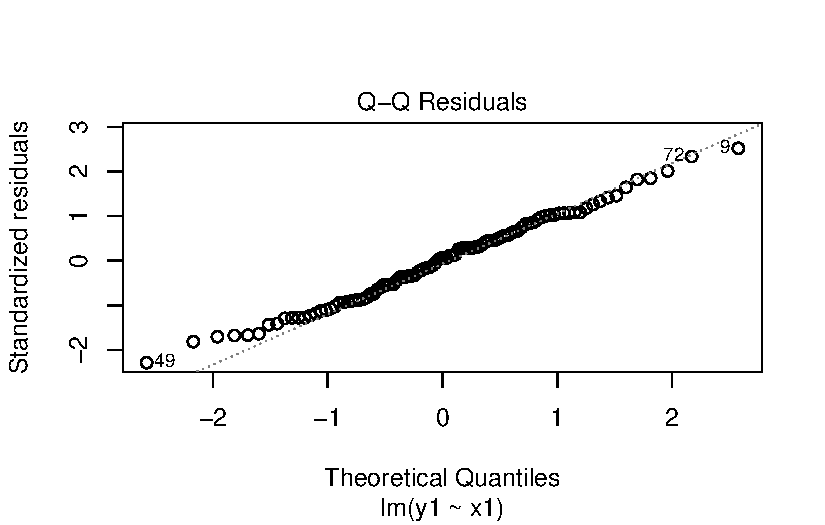
\includegraphics[keepaspectratio]{Week2_exerc_sol_files/figure-pdf/unnamed-chunk-2-3.pdf}}

\begin{Shaded}
\begin{Highlighting}[]
\CommentTok{\# For the binary explanatory variable x2}
\FunctionTok{boxplot}\NormalTok{(y1 }\SpecialCharTok{\textasciitilde{}}\NormalTok{ x2, }\AttributeTok{data =}\NormalTok{ assumptions)}
\end{Highlighting}
\end{Shaded}

\pandocbounded{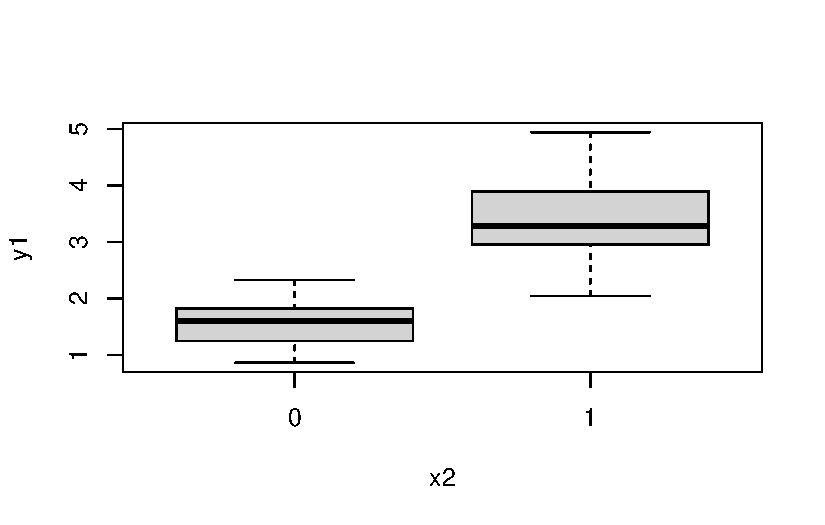
\includegraphics[keepaspectratio]{Week2_exerc_sol_files/figure-pdf/unnamed-chunk-2-4.pdf}}

\begin{Shaded}
\begin{Highlighting}[]
\FunctionTok{aggregate}\NormalTok{( y1 }\SpecialCharTok{\textasciitilde{}}\NormalTok{ x2, }\AttributeTok{data =}\NormalTok{ assumptions, }\AttributeTok{FUN =}\NormalTok{ sd) }\CommentTok{\# Calculates the standard deviation in each group}
\end{Highlighting}
\end{Shaded}

\begin{verbatim}
  x2        y1
1  0 0.3687492
2  1 0.7036609
\end{verbatim}

\begin{Shaded}
\begin{Highlighting}[]
\NormalTok{y1\_x2\_reg }\OtherTok{\textless{}{-}} \FunctionTok{lm}\NormalTok{(y1 }\SpecialCharTok{\textasciitilde{}}\NormalTok{ x2, }\AttributeTok{data =}\NormalTok{ assumptions) }\CommentTok{\# Carry out regression}
\FunctionTok{plot}\NormalTok{(y1\_x2\_reg, }\DecValTok{2}\NormalTok{)  }\CommentTok{\# Normal quantile plot of residuals}
\end{Highlighting}
\end{Shaded}

\pandocbounded{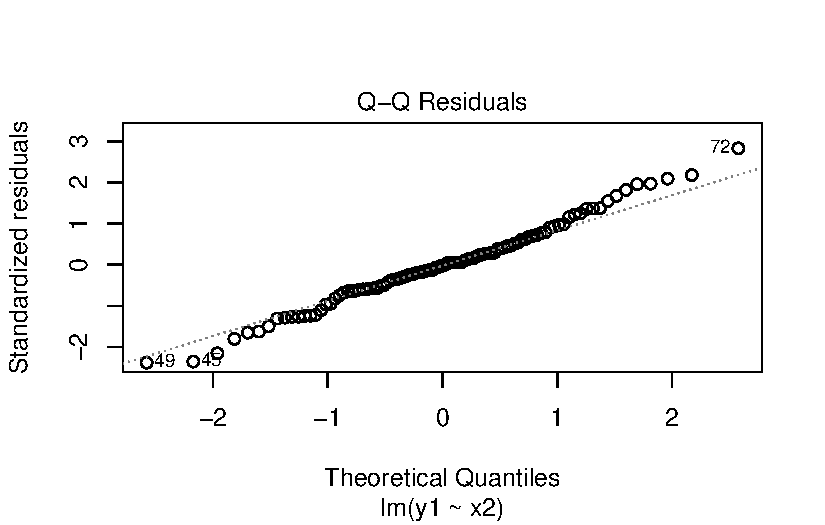
\includegraphics[keepaspectratio]{Week2_exerc_sol_files/figure-pdf/unnamed-chunk-2-5.pdf}}

:::

\subsubsection{Regression between y1 and
x1}\label{regression-between-y1-and-x1}

The residua versus fitted plot shows that the linearity assumption is
violated in this data. This is because residuals are generally positive
for low and high values of \texttt{x}, and negative for mid range
\texttt{x} values. The violation of linearity here makes
homoscedasticity more difficult to assess, however as there is no
obvious fanning in the residuals, this assumption has been met. The
normal quantile plot shows no evidence for a concerning deviation from
normality, so the normality of residuals assumption is met.

\subsubsection{Regression between y2 and
x1}\label{regression-between-y2-and-x1}

The residual versus fitted plot shows that the linearity assumption is
met in this data. This is because the residuals are generally scattered
around zero for all fitted values. The fanning out pattern in this plot
however show that the residual error is increasing for larger fitted
values. This shows that that homoscedasticity assumption is violated.
The normality of residuals assumption has been met as demonstrated by a
reasonably straight line in the normal quantile plot.

\subsubsection{Regression between y3 and
x1}\label{regression-between-y3-and-x1}

The residual versus fitted plot shows an even scatter around zero for
all fitted values that neither fans in our out. Therefore linearity and
homoscedasticity are met in this regression. The normal quantile plot
also follows a very straight line, showing that the normality of
residual assumption has been met.

\subsubsection{Regression between y4 and
x1}\label{regression-between-y4-and-x1}

The residual versus fitted plot is a little strange on this one. There
is on evidence of non-linearity (the residauls don't trend upwards or
downwards), and there is no evidence of hetergeniety (as the scatter
doesn't fan in or out). However there are larger positive valued
residuals than negative valued residuals. This is indicating that the
residuals are skewed. The normal quantile plot confirms this with strong
departures from normality. This is also evident in a histogram of
residuals.

\subsubsection{Regression between y1 and
x2}\label{regression-between-y1-and-x2}

The boxplot shows different variances for each value of \texttt{x2}, so
it looks like homoscedasticity might be violated here. The standard
deviation is each group is 0.37 and 0.70 - confirming heterogeneity. As
\texttt{x2} is categorical, we do not need to check linearity. The
normal quantile plot of the residuals shows some departures of normality
towards the tails, but is reasonably fine - so this assumption is met.

\subsubsection{Regression between y2 and
x2}\label{regression-between-y2-and-x2}

The boxplot shows different variances for each value of \texttt{x2}, so
it looks like homoscedasticity might be violated here. The standard
deviation is each group is 0.28 and 0.48 - confirming heterogeneity. As
\texttt{x2} is categorical, we do not need to check linearity. The
normal quantile plot of the residuals is fairly straight, and so the
assumption of normality is met.

\subsubsection{Regression between y3 and
x2}\label{regression-between-y3-and-x2}

The bloxplot show relative similar variances for each value of
\texttt{x2} - so it looks like the homoscedasticity assumption is met
here. The calculated standard deviation in each group is 0.34 and 0.39 -
a relatively small difference that may be attributable to random
variation. So the homoscedasticity assumption is met. As \texttt{x2} is
categorical, we do not need to check linearity. The normal quantile plot
of the residuals is fairly straight, and so the assumption of normality
is met.

\subsubsection{Regression between y4 and
x2}\label{regression-between-y4-and-x2}

The bloxplot show relative similar variances for each value of
\texttt{x2} - so it looks like the homoscedasticity assumption is met
here. The calculated standard deviation in each group is 0.22 and 0.27.
The boxplot also shows a few high value outliers, that may indicate the
data is skewed. The normal quantile plot does show some departure from
normality (particularly for the larger quantiles), but it isn't too
extreme. Given the reasonably large dataset (100 observations), the
central limit theorem will ensure that a simple linear regression is
appropriate here, even with some small depature from normality of the
residuals.




\end{document}
